%
% fw.tex -- Durchführung des Floyd-Warshall Algorithmus
%
% (c) 2019 Prof Dr Andreas Müller, Hochschule Rapperswil
%
\bgroup

\definecolor{wegelb}{rgb}{1,0.6,0}
\definecolor{weghell}{rgb}{1,0.9,0.6}
\definecolor{darkgreen}{rgb}{0,0.6,0}

\begin{columns}[t]
\begin{column}{0.44\hsize}
\begin{center}
\begin{tikzpicture}[>=latex]


\def\r{2.2}
\coordinate (A) at ({\r*cos(-54+0*72)},{\r*sin(-54+0*72)});
\coordinate (C) at ({\r*cos(-54+1*72)},{\r*sin(-54+1*72)});
\coordinate (D) at ({\r*cos(-54+2*72)},{\r*sin(-54+2*72)});
\coordinate (B) at ({\r*cos(-54+3*72)},{\r*sin(-54+3*72)});
\coordinate (E) at ({\r*cos(-54+4*72)},{\r*sin(-54+4*72)});

\def\knoten#1#2#3{
	\fill[color=#3] #1 circle[radius=0.3];
	\draw[line width=1pt] #1 circle[radius=0.3];
	\node at #1 {$#2$};
}

\def\kante#1#2#3{
	\draw[->,line width=1pt,shorten >= 0.3cm,shorten <= 0.3cm] #1 -- #2;
	\fill[color=white,opacity=0.7] ($0.5*#1+0.5*#2$) circle[radius=0.22];
	\node at ($0.5*#1+0.5*#2$) {$#3$};
}

% Wege über 1
% 3--1--5
\only<4>{
	\draw[->,line width=7pt,color=red!50] 
		(C)--(A)--(E);
}

% Wege über 2
% 5--2--3
\only<6>{
	\draw[->,line width=7pt,color=red!50] 
		(E)--(B)--(C);
}
% 5--2--4
\only<7>{
	\draw[->,line width=7pt,color=red!50] 
		(E)--(B)--(D);
	\draw[->,line width=7pt,color=blue!50,dashed] 
		(E)--(D);
}

% Wege über 3
% 2--3--1
\only<9>{
	\draw[->,line width=7pt,color=red!50] 
		(B)--(C)--(A);
}
% 2--3--5
\only<10>{
	\draw[->,line width=7pt,color=red!50] 
		(B)--(C)--(A)--(E);
}
% 4--3--1
\only<11>{
	\draw[->,line width=7pt,color=red!50] 
		(D)--(C)--(A);
}
% 4--3--5
\only<12>{
	\draw[->,line width=7pt,color=red!50] 
		(D)--(C)--(A)--(E);
}
% 5--3--1
\only<13>{
	\draw[->,line width=7pt,color=red!50] 
		(E)--(B)--(C)--(A);
}
% 5--3--5
\only<14>{
	\draw[->,line width=7pt,color=red!50] 
		(E)--(B)--(C)--(A)--(E);
}

% Wege über 4
% 2--4--1
\only<16>{
	\draw[->,line width=7pt,color=red!50] 
		(B)--(D)--(C)--(A);
	\draw[->,line width=7pt,color=blue!50,dashed] 
		(B)--(C)--(A);
}
% 2--4--3
\only<17>{
	\draw[->,line width=7pt,color=red!50] 
		(B)--(D)--(C);
	\draw[->,line width=7pt,color=blue!50,dashed] 
		(B)--(C);
}
% 2--4--5
\only<18>{
	\draw[->,line width=7pt,color=red!50] 
		(B)--(D)--(C)--(A)--(E);
	\draw[->,line width=7pt,color=blue!50,dashed] 
		(B)--(C)--(A)--(E);
}
% 5--4--1
\only<19>{
	\draw[->,line width=7pt,color=red!50] 
		(E)--(D)--(C)--(A);
	\draw[->,line width=7pt,color=blue!50,dashed] 
		(E)--(B)--(C)--(A);
}
% 5--4--3
\only<20>{
	\draw[->,line width=7pt,color=red!50] 
		(E)--(D)--(C);
	\draw[->,line width=7pt,color=blue!50,dashed] 
		(E)--(B)--(C);
}
% 5--4--5
\only<21>{
	\draw[->,line width=7pt,color=red!50] 
		(E)--(D)--(C)--(A)--(E);
	\draw[->,line width=7pt,color=blue!50,dashed] 
		(E)--(B)--(C)--(A)--(E);
}
% 1--5--1
\only<23>{
	\draw[->,line width=7pt,color=red!50] 
		(A)--(E)--(B)--(C)--(A);
}
% 1--5--2
\only<24>{
	\draw[->,line width=7pt,color=red!50] 
		(A)--(E)--(B);
}
% 1--5--3
\only<25>{
	\draw[->,line width=7pt,color=red!50] 
		(A)--(E)--(B)--(C);
}
% 1--5--4
\only<26>{
	\draw[->,line width=7pt,color=red!50] 
		(A)--(E)--(D);
}
% 2--5--1
\only<27>{
	\draw[->,line width=7pt,color=red!50] 
		(B)--(C)--(A)--(E)--(D)--(C)--(A);
	\draw[->,line width=7pt,color=blue!50,dashed] 
		(B)--(C)--(A);
}
% 2--5--2
\only<28>{
	\draw[->,line width=7pt,color=red!50] 
		(B)--(C)--(A)--(E)--(B);
}
% 2--5--3
\only<29>{
	\draw[->,line width=7pt,color=red!50] 
		(B)--(C)--(A)--(E)--(D)--(C);
	\draw[->,line width=7pt,color=blue!50,dashed] 
		(B)--(C);
}
% 2--5--4
\only<30>{
	\draw[->,line width=7pt,color=red!50] 
		(B)--(C)--(A)--(E)--(D);
	\draw[->,line width=7pt,color=blue!50,dashed] 
		(B)--(D);
}
% 3--5--1
\only<31>{
	\draw[->,line width=7pt,color=red!50] 
		(C)--(A)--(E)--(D)--(C)--(A);
	\draw[->,line width=7pt,color=blue!50,dashed] 
		(C)--(A);
}
% 3--5--2
\only<32>{
	\draw[->,line width=7pt,color=red!50] 
		(C)--(A)--(E)--(B);
}
% 3--5--3
\only<33>{
	\draw[->,line width=7pt,color=red!50] 
		(C)--(A)--(E)--(B)--(C);
}
% 3--5--4
\only<34>{
	\draw[->,line width=7pt,color=red!50] 
		(C)--(A)--(E)--(D);
}
% 4--5--1
\only<35>{
	\draw[->,line width=7pt,color=red!50] 
		(D)--(C)--(A)--(E)--(D)--(C)--(A);
	\draw[->,line width=7pt,color=blue!50,dashed] 
		(D)--(C)--(A);
}
% 4--5--2
\only<36>{
	\draw[->,line width=7pt,color=red!50] 
		(D)--(C)--(A)--(E)--(B);
}
% 4--5--3
\only<37>{
	\draw[->,line width=7pt,color=red!50] 
		(D)--(C)--(A)--(E)--(D)--(C);
	\draw[->,line width=7pt,color=blue!50,dashed] 
		(D)--(C);
}
% 4--5--4
\only<38>{
	\draw[->,line width=7pt,color=red!50] 
		(D)--(C)--(A)--(E)--(D);
}


\uncover<40>{
	\draw[->,color=red!50,line width=7pt]
		(B)--(C)--(A)--(E)--(D);
}

\kante{(A)}{(E)}{1}
\kante{(B)}{(C)}{2}
\kante{(B)}{(D)}{13}
\kante{(C)}{(A)}{3}
\kante{(D)}{(C)}{6}
\kante{(E)}{(B)}{5}
\kante{(E)}{(D)}{6}

\only<1>{
	\knoten{(A)}{}{white}
	\knoten{(B)}{}{white}
	\knoten{(C)}{}{white}
	\knoten{(D)}{}{white}
	\knoten{(E)}{}{white}
}

\only<2->{
	\knoten{(A)}{1}{white}
	\knoten{(B)}{2}{white}
	\knoten{(C)}{3}{white}
	\knoten{(D)}{4}{white}
	\knoten{(E)}{5}{white}
}

\only<4>{
	\knoten{(A)}{1}{darkgreen!50}
}
\only<6-7>{
	\knoten{(B)}{2}{darkgreen!50}
}
\only<9-14>{
	\knoten{(C)}{3}{darkgreen!50}
}
\only<16-21>{
	\knoten{(D)}{4}{darkgreen!50}
}
\only<23-38>{
	\knoten{(E)}{5}{darkgreen!50}
}

\end{tikzpicture}
\end{center}
\begin{block}{Aufgabe}
Finde den kürzesten Weg von 2 nach 4
\end{block}
\end{column}
\begin{column}{0.5\hsize}
\begin{center}
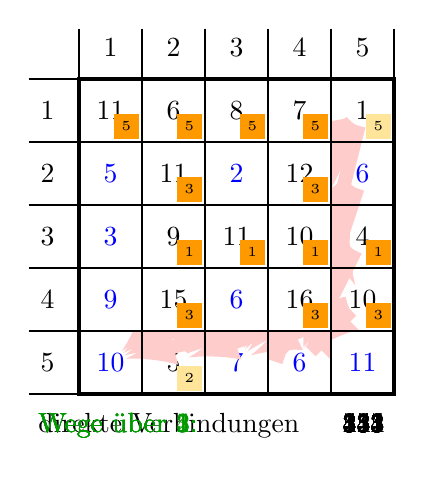
\begin{tikzpicture}[>=latex,scale=0.8]

\def\punkt#1#2{
	({#2-0.5},{0.5-(#1)})
}
\def\punktoff#1#2{
	({#2-0.7},{0.7-(#1)})
}
\def\feld#1#2#3{
	\ifthenelse{\boolean{wegweiser}}{
		\fill[color=white]
			({#2-1},{1-#1}) rectangle ({#2-0.45},{0.45-#1});
		\node at \punktoff{#1}{#2} {$#3$};
	}{
		\fill[color=white]
			({#2-1},{1-#1}) rectangle ({#2},{-#1});
		\node at \punkt{#1}{#2} {$#3$};
	}
}
\def\verbindung#1#2#3{
	\draw[->,line width=5pt,color=red!20,shorten >= 0.2cm,shorten <= 0.2cm]
		\punkt{#1}{#2}--\punkt{#2}{#3};
	\node at (5,-5.5) [left] {$#1\rightsquigarrow #2\rightsquigarrow #3$\strut};
}
\def\Infty{{}}
\def\wegweiser#1#2#3{
	\ifthenelse{\boolean{wegweiser}}{
		\ifnum #2 = #3
		\fill[color=weghell]
			({#2-0.45},{0.45-#1}) rectangle ({#2-0.05},{0.05-#1});
		\else
		\fill[color=wegelb]
			({#2-0.45},{0.45-#1}) rectangle ({#2-0.05},{0.05-#1});
		\fi
		\node at ({#2-0.25},{0.25-#1}) {\tiny #3};
	}{}
}

% direkte Wege
\uncover<3->{
	\feld{1}{1}{\Infty}
	\feld{1}{2}{\Infty}
	\feld{1}{3}{\Infty}
	\feld{1}{4}{\Infty}
	\feld{1}{5}{1}
	\wegweiser{1}{5}{5}

	\feld{2}{1}{\Infty}
	\feld{2}{2}{\Infty}
	\feld{2}{3}{2}
	\wegweiser{2}{3}{3}
	\feld{2}{4}{13}
	\wegweiser{2}{4}{4}
	\feld{2}{5}{\Infty}

	\feld{3}{1}{3}
	\wegweiser{3}{1}{1}
	\feld{3}{2}{\Infty}
	\feld{3}{3}{\Infty}
	\feld{3}{4}{\Infty}
	\feld{3}{5}{\Infty}

	\feld{4}{1}{\Infty}
	\feld{4}{2}{\Infty}
	\feld{4}{3}{6}
	\wegweiser{4}{3}{3}
	\feld{4}{4}{\Infty}
	\feld{4}{5}{\Infty}

	\feld{5}{1}{\Infty}
	\feld{5}{2}{5}
	\wegweiser{5}{2}{2}
	\feld{5}{3}{\Infty}
	\feld{5}{4}{6}
	\wegweiser{5}{4}{4}
	\feld{5}{5}{\Infty}
}

\uncover<3-3>{
	\node at (-0.8,-5.5) [right] {direkte Verbindungen};
}

\uncover<4-4>{
	\node[color=darkgreen] at (-0.8,-5.5) [right] {Wege über $1$:\strut};
}

% Wege über 1
% 3-1-5
\uncover<4>{
	\verbindung{3}{1}{5}
	\feld{3}{5}{\color{red}4}
	\wegweiser{3}{5}{1}
}
\uncover<5->{
	\feld{3}{5}{4}
	\wegweiser{3}{5}{1}
}

\uncover<6-7>{
	\node[color=darkgreen] at (-0.8,-5.5) [right] {Wege über $2$:\strut};
}

% Wege über 2
% 5-2-3
\uncover<6>{
	\verbindung{5}{2}{3}
	\feld{5}{3}{\color{red}7}
	\wegweiser{5}{3}{2}
}
\uncover<7->{
	\feld{5}{3}{7}
	\wegweiser{5}{3}{2}
}
% 5-2-4
\uncover<7>{
	\verbindung{5}{2}{4}
	\feld{5}{4}{\color{blue}6}
}

\uncover<9-14>{
	\node[color=darkgreen] at (-0.8,-5.5) [right] {Wege über $3$:\strut};
}

% Wege über 3
% 2-3-1
\uncover<9>{
	\verbindung{2}{3}{1}
	\feld{2}{1}{\color{red}5}
	\wegweiser{2}{1}{3}
}
\uncover<10->{
	\feld{2}{1}{5}
	\wegweiser{2}{1}{3}
}
% 2-3-5
\uncover<10>{
	\verbindung{2}{3}{5}
	\feld{2}{5}{\color{red}6}
	\wegweiser{2}{5}{3}
}
\uncover<11->{
	\feld{2}{5}{6}
	\wegweiser{2}{5}{3}
}
% 4-3-1
\uncover<11>{
	\verbindung{4}{3}{1}
	\feld{4}{1}{\color{red}9}
	\wegweiser{4}{1}{3}
}
\uncover<12->{
	\feld{4}{1}{9}
	\wegweiser{4}{1}{3}
}
% 4-3-5
\uncover<12>{
	\verbindung{4}{3}{5}
	\feld{4}{5}{\color{red}10}
	\wegweiser{4}{5}{3}
}
\uncover<13->{
	\feld{4}{5}{10}
	\wegweiser{4}{5}{3}
}
% 5-3-1
\uncover<13>{
	\verbindung{5}{3}{1}
	\feld{5}{1}{\color{red}10}
	\wegweiser{5}{1}{2}
}
\uncover<14->{
	\feld{5}{1}{10}
	\wegweiser{5}{1}{2}
}
% 5-3-5
\uncover<14>{
	\verbindung{5}{3}{5}
	\feld{5}{5}{\color{red}11}
	\wegweiser{5}{5}{2}
}
\uncover<15->{
	\feld{5}{5}{11}
	\wegweiser{5}{5}{2}
}

\uncover<16-21>{
	\node[color=darkgreen] at (-0.8,-5.5) [right] {Wege über $4$:\strut};
}

% Wege über 4
% 2-4-1
\uncover<16>{
	\verbindung{2}{4}{1}
	\feld{2}{1}{\color{blue}5}
}
% 2-4-3
\uncover<17>{
	\verbindung{2}{4}{3}
	\feld{2}{3}{\color{blue}2}
}
% 2-4-5
\uncover<18>{
	\verbindung{2}{4}{5}
	\feld{2}{5}{\color{blue}6}
}
% 5-4-1
\uncover<19>{
	\verbindung{5}{4}{1}
	\feld{5}{1}{\color{blue}10}
}
% 5-4-3
\uncover<20>{
	\verbindung{5}{4}{3}
	\feld{5}{3}{\color{blue}7}
}
% 5-4-5
\uncover<21>{
	\verbindung{5}{4}{5}
	\feld{5}{5}{\color{blue}11}
}

% Wege über 5
\uncover<23-38>{
	\node[color=darkgreen] at (-0.8,-5.5) [right] {Wege über $5$:\strut};
}

% Wege über 5
% 1-5-1
\uncover<23>{
	\verbindung{1}{5}{1}
	\feld{1}{1}{\color{red}11}
	\wegweiser{1}{1}{5}
}
\uncover<24->{
	\feld{1}{1}{11}
	\wegweiser{1}{1}{5}
}
% 1-5-2
\uncover<24>{
	\verbindung{1}{5}{2}
	\feld{1}{2}{\color{red}6}
	\wegweiser{1}{2}{5}
}
\uncover<25->{
	\feld{1}{2}{6}
	\wegweiser{1}{2}{5}
}
% 1-5-3
\uncover<25>{
	\verbindung{1}{5}{3}
	\feld{1}{3}{\color{red}8}
	\wegweiser{1}{3}{5}
}
\uncover<26->{
	\feld{1}{3}{8}
	\wegweiser{1}{3}{5}
}
% 1-5-4
\uncover<26>{
	\verbindung{1}{5}{4}
	\feld{1}{4}{\color{red}7}
	\wegweiser{1}{4}{5}
}
\uncover<27->{
	\feld{1}{4}{7}
	\wegweiser{1}{4}{5}
}
% 2-5-1
\uncover<27>{
	\verbindung{2}{5}{1}
	\feld{2}{1}{\color{blue}5}
}
% 2-5-2
\uncover<28>{
	\verbindung{2}{5}{2}
	\feld{2}{2}{\color{red}11}
	\wegweiser{2}{2}{3}
}
\uncover<29->{
	\feld{2}{2}{11}
	\wegweiser{2}{2}{3}
}
% 2-5-3
\uncover<29>{
	\verbindung{2}{5}{3}
	\feld{2}{3}{\color{blue}2}
}
% 2-5-4
\uncover<30>{
	\verbindung{2}{5}{4}
	\feld{2}{4}{\color{red}12}
	\wegweiser{2}{4}{3}
}
\uncover<31->{
	\feld{2}{4}{12}
	\wegweiser{2}{4}{3}
}
% 3-5-1
\uncover<31>{
	\verbindung{3}{5}{1}
	\feld{3}{1}{\color{blue}3}
}
% 3-5-2
\uncover<32>{
	\verbindung{3}{5}{2}
	\feld{3}{2}{\color{red}9}
	\wegweiser{3}{2}{1}
}
\uncover<33->{
	\feld{3}{2}{9}
	\wegweiser{3}{2}{1}
}
% 3-5-3
\uncover<33>{
	\verbindung{3}{5}{3}
	\feld{3}{3}{\color{red}11}
	\wegweiser{3}{3}{1}
}
\uncover<34->{
	\feld{3}{3}{11}
	\wegweiser{3}{3}{1}
}
% 3-5-4
\uncover<34>{
	\verbindung{3}{5}{4}
	\feld{3}{4}{\color{red}10}
	\wegweiser{3}{4}{1}
}
\uncover<35->{
	\feld{3}{4}{10}
	\wegweiser{3}{4}{1}
}
% 4-5-1
\uncover<35>{
	\verbindung{4}{5}{1}
	\feld{4}{1}{\color{blue}9}
}
% 4-5-2
\uncover<36>{
	\verbindung{4}{5}{2}
	\feld{4}{2}{\color{red}15}
	\wegweiser{4}{2}{3}
}
\uncover<37->{
	\feld{4}{2}{15}
	\wegweiser{4}{2}{3}
}
% 4-5-3
\uncover<37>{
	\verbindung{4}{5}{3}
	\feld{4}{3}{\color{blue}6}
}
% 4-5-4
\uncover<38>{
	\verbindung{4}{5}{4}
	\feld{4}{4}{\color{red}16}
	\wegweiser{4}{4}{3}
}
\uncover<39->{
	\feld{4}{4}{16}
	\wegweiser{4}{4}{3}
}


\uncover<3->{

	\foreach \x in {0,...,5}{
		\draw[line width=0.7pt] (\x,0.8)--(\x,-5);
	}
	\foreach \y in {0,...,-5}{
		\draw[line width=0.7pt] (-0.8,\y)--(5,\y);
	}
	\draw[line width=1.4pt] (0,0)--(5,0)--(5,-5)--(0,-5)--cycle;

	\node at (0.5,0.5) {$1$};
	\node at (1.5,0.5) {$2$};
	\node at (2.5,0.5) {$3$};
	\node at (3.5,0.5) {$4$};
	\node at (4.5,0.5) {$5$};

	\node at (-0.5,-0.5) {$1$};
	\node at (-0.5,-1.5) {$2$};
	\node at (-0.5,-2.5) {$3$};
	\node at (-0.5,-3.5) {$4$};
	\node at (-0.5,-4.5) {$5$};
}

\end{tikzpicture}
\end{center}

\uncover<40>{
	\vspace{-22pt}
	\begin{block}{Lösung}
	Der kürzeste Weg von 2 nach 4 ist 2---3---1---5---4
	\end{block}
}

\end{column}
\end{columns}

\egroup
